\documentclass[11pt, a4paper]{article}

\usepackage[english]{babel}
\usepackage{sleek}
\usepackage{common}

\title{INFO8006 - Introduction to Artificial Intelligence}
\subtitle{Exercise session 1}

\def\Astar{$\text{A}^*$}

\begin{document}

\maketitle

\begin{thbox}{Search problem formulation}
    A \thighlight{search problem} is defined by    
    \begin{itemize}
        \item A representation for \thighlight{states}.
        \item The \thighlight{initial} state of the agent.
        \item A set of \thighlight{actions} allowed in every state \thighlight{$s$}.
        \item A \thighlight{transition model $s' = result(s,a)$} that returns the resulting state \thighlight{$s'$} for using action \thighlight{$a$} in state \thighlight{$s$}. 
        \item A \thighlight{goal test} which determines if the problem is solved in state \thighlight{$s$}.
        \item A \thighlight{path cost} that assigns a numerical cost to each path. We assume the later to be a sum of positive step costs \thighlight{$c(s,a,s')$} along the path. 
    \end{itemize}
\end{thbox}

\begin{thbox}{Searching strategy}
\begin{itemize}[leftmargin=*]
    \item \textbf{Depth-First Search} uses a stack (LIFO) for the \thighlight{\textit{fringe}}.
    \item \textbf{Breadth-First Search} uses a queue (FIFO) for the \thighlight{\textit{fringe}}.
    \item \textbf{Uniform-Cost Search} uses a priority queue for the \thighlight{\textit{fringe}},\\where the priority is the \thighlight{cumulative cost $g(n)$}.
    \item \textbf{Greedy Search} uses a priority queue for the \thighlight{\textit{fringe}},\\where the priority is a \thighlight{heuristic $h(n)$}.
    \item \textbf{A* Search} uses a priority queue for the \thighlight{\textit{fringe}},\\where the priority is the sum of both \thighlight{heuristic $h(n)$ and cumulative cost $g(n)$}.
\end{itemize}
\end{thbox}

\begin{thbox}{Heuristic}
    A \thighlight{heuristic function $h(n)$} estimates the cost of the cheapest path from node \thighlight{$n$} to a goal state.\\
    A \thighlight{heuristic} is \thighlight{admissible} if
    $$0 \leq h(n) \leq h^*(n)$$
    with $h^*(n)$ being the tightest \thighlight{heuristic}, i.e. the true \thighlight{cumulative cost}.\\
    A \thighlight{heuristic} is \thighlight{consistent} if
    $$h(n) \leq c(n,a,n') + h(n')$$
    for all node-action-resulting node triplets \thighlight{$(n,a,n')$}.
\end{thbox}

\begin{figure}[h]
    \centering
    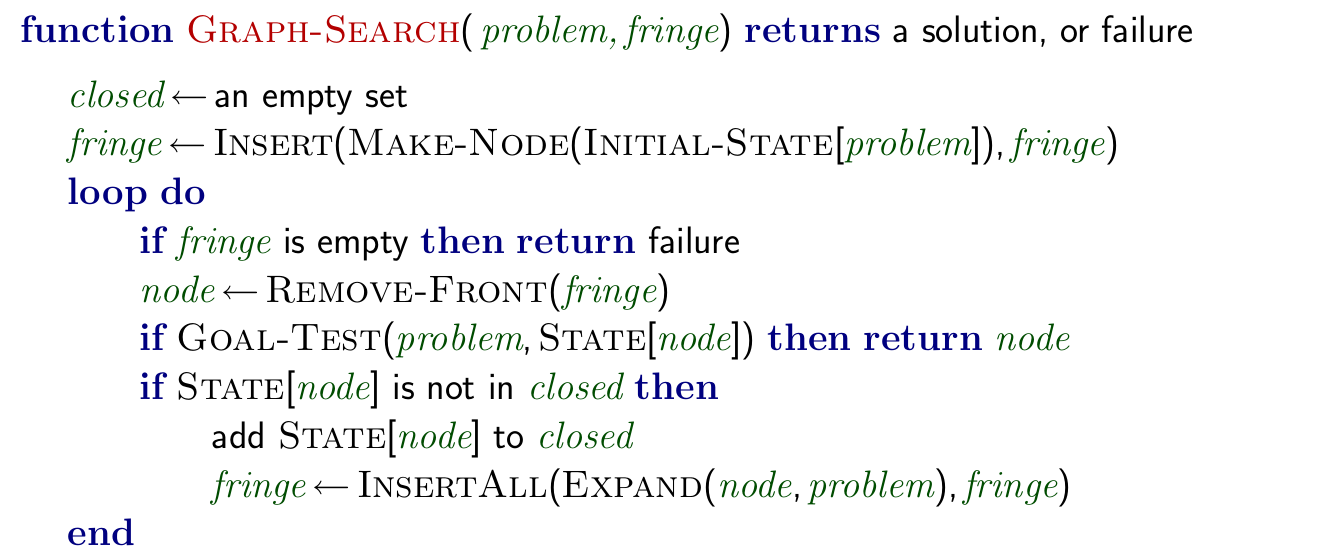
\includegraphics[width=.9\linewidth]{figures/graph-search.png}
\end{figure}


\textbf{In session exercises:} Ex. 1, Ex. 2.1-3-4 

\newpage

\section{Path finding}

Tram'Ardent deployed a new robot to help them on the finishing touches of Liège worksite. This robot's goal is to convey weeds that were removed by the gardeners to a container as fast as possible. Assuming that 
\begin{itemize}
    \item the fuel cost used by the robot is negligible
    \item the robot can only navigate on guides that are placed in a rectangular grid configuration and can locate itself on the grid
    \item there is only one pile and one container by zone (i.e. by grid) for which positions are known by the robot
    \item the speed of the robot is constant and the grass loading/unloading is instantaneous
    \item the robot can only carry a limited weight of grass at once
    % \item some nodes on the grid take twice the time to cross because the terrain is rugged
    \item the robot can know the initial weight of grass on the pile.
\end{itemize}
For a given grid

\begin{enumerate}
    \item Formulate a corresponding search problem.
    
    \begin{solution}
        \textbf{State representation}: Assuming a $H\times W$ grid, the state is represented by the position $(i,j) \in \{1,...,W\}\times \{1,...,H\}$ of the robot, the remaining weight of grass $w_G$ and a flag $L$ indicating whether the robot is loaded or not. Following other assumptions, we also define the location of the pile and the container respectively by $P = (i_p,j_p)$ and $C = (i_c,j_c)$ as well as the weight limit of the robot $w_{max}$.\\
        
        \textbf{Initial state}: No specific information is given, we can assume it starts anywhere on the grid, unloaded. $s_0 = (i_0, j_0, w_{G0}, False)$\\
        
        \textbf{Actions}: $a \in \{LEFT, UP, RIGHT, DOWN\}$\\
        
        \textbf{Transition model}: \[(i,j)' = \begin{cases*}
            (i+1,j)\ &\text{if $a = RIGHT$ and $i < W$}\\
            (i,j+1)\ &\text{if $a = UP$ and $j < H$}\\
            (i-1,j)\ &\text{if $a = LEFT$ and $i > 1$}\\
            (i,j-1)\ &\text{if $a = DOWN$ and $j > 1$}\\
            (i,j)\ &\text{otherwise}
        \end{cases*}\]\\
        \[w_G' = \begin{cases*}
            w_G - min(w_G, w_{max})\ &\text{if $(i,j)' == P$}\\
            w_G\ &\text{otherwise}
        \end{cases*}\]\\
        \[L' = \begin{cases*}
            \text{\textbf{True} if $L$ and $(i,j)' \not = C$}\\
            \text{\textbf{True} if $w_G > 0$ and $(i,j)' == P$}\\
            \text{\textbf{False} otherwise}
        \end{cases*}\]\\
        
        \textbf{Goal test}: $goal(s) = \text{ not }L$ and $w_G == 0$\\
        
        \textbf{Step cost}: Under the given assumptions, every step from one node to another is equivalent. Then $c(s,a,s') = 1$ is relevant. Note that it could be any constant step cost.\\
    \end{solution}
    \item Knowing that the terrain can be rugged at specific places, causing slow down of the robot, propose an admissible heuristic which estimates the remaining cost at any node.
    
    \begin{solution}
        As usual, in grid problem, Manhattan distance or Euclidean distance is admissible as long as the step cost is 1 everywhere\footnote{Choosing a constant step cost $K > 1$ does not break admissibility in this case. If $K \in [0,1[$, then $h(s)$ is not admissible but $Kh(s)$ is.}. However, the robot can go back and forth if $w_G > w_{max}$. Then an admissible heuristic would be
        \[h(s) = \begin{cases*}
            |i_c - i| + |j_c - j| + 2\ceil{\frac{w_G}{w_{max}}}\big(|i_c - i_p| + |j_c - j_p|\big)\ &\text{if $L$}\\
            |i_p - i| + |j_p - j| + \big(2\ceil{\frac{w_G}{w_{max}}} - 1\big)\big(|i_c - i_p| + |j_c - j_p|\big)\ &\text{if not $L$}
        \end{cases*}\]
        which would have been the true remaining cost if the terrain was not rugged.
    \end{solution}

    \item Now the robot can move in diagonal. Is your heuristic still admissible? If not, what should you change? What if the robot is twice as fast diagonally?

    \begin{solution}
        The Manhattan distance cannot be used anymore, only the Euclidean distance would be admissible (amongst the previous proposals) or any other function dominated by the Euclidean distance.\\
        If the robot moves in diagonal twice faster, you should divide the distance by a factor 2 (equivalent to say that the cost is 0.5 in diagonals). The most limiting case being a perfect diagonal going from $P$ to $C$.
    \end{solution}
\end{enumerate}

\newpage 

\section{Search algorithms}

\begin{figure}[h]
    \centering
    \scalebox{0.75}{\begin{tikzpicture}[node distance = 4cm]
        \node[state] (S) {S(tart)\\$h=11$};
        \node[state] (A) [above right of=S] {A\\$h=20$};
        \node[state] (B) [right of=S] {B\\$h=12$};
        \node[state] (C) [below right of=S] {C\\$h=10$};
        \node[state] (D) [below right of=B] {D\\$h=3$};
        \node[state] (E) [above right of=B] {E\\$h=19$};
        \node[state] (G) [right of=D] {G(oal)};

        \path[-] (S) edge node[fill=white] {1} (A);
        \path[-] (S) edge node[fill=white] {4} (B);
        \path[-] (S) edge node[fill=white] {3} (C);
        \path[-] (B) edge node[fill=white] {7} (D);
        \path[-] (B) edge node[fill=white] {5} (E);
        \path[-] (D) edge node[fill=white] {10} (G);
        \path[-] (E) edge node[fill=white] {1} (D);
        \path[-] (E) edge node[fill=white] {20} (G);
        \path[-] (C) edge node[fill=white] {2} (B);
        \path[-] (A) edge node[fill=white] {5} (B);
    \end{tikzpicture}}
\end{figure}

For each of the following search algorithms, apply the \textsc{Graph-Search} algorithm (lecture 2, slide 62) and give the order in which the states, represented by the nodes of this undirected graph, are expanded, as well as the final path returned by the algorithm. If two nodes are in competition to be expanded, the conflict is resolved by alphabetical order.

% \begin{solution}
%     \newpage
% \end{solution}

\begin{enumerate}
    \item Depth-First Search (DFS)

    \begin{solution}
        We use a Last-In First-Out (LIFO) fringe, \ie{} a \emph{stack}, to perform the search. In this stack, we keep track of the states that are reachable from the visited (closed) states. These states are annotated with the state they were expanded from, which allows to reconstruct the path at the end. At each step, the state at the \emph{top} of the stack is \emph{popped}. If it was not visited previously, it is expanded, which consists in \emph{pushing} its neighbors to the \emph{top} of the stack.

        \begin{table}[H]
            \centering
            \begin{tabular}{l|l}
                \toprule
                Fringe (LIFO stack) & Closed \\
                \midrule
                S & \\
                C(S) B(S) A(S) & S \\
                C(S) B(S) B(A) & S A \\
                C(S) B(S) E(B) D(B) C(B) & S A B \\
                C(S) B(S) E(B) D(B) & S A B C \\
                C(S) B(S) E(B) G(D) E(D) & S A B C D \\
                C(S) B(S) E(B) G(D) G(E) & S A B C D E \\
                \bottomrule
            \end{tabular}
        \end{table}

        For readability, nodes that are already in the closed set are not added to the fringe.

        Expansion: S, A, B, C, D, E, G. Path: S, A, B, D, E, G.
    \end{solution}

    \item Breadth-First Search (BFS)

    \begin{solution}
        We use a First-In First-Out (FIFO) fringe, \ie{} a \emph{queue}, to keep track of the reachable states. At each step, the state at the \emph{front} of the queue is popped. If it was not visited previously, it is expanded, which consists in pushing its neighbors to the \emph{back} of the queue.

        \begin{table}[h]
            \centering
            \begin{tabular}{l|l}
                \toprule
                Fringe (FIFO queue) & Closed \\
                \midrule
                S & \\
                C(S) B(S) A(S) & S \\
                B(A) C(S) B(S) & S A \\
                E(B) D(B) C(B) B(A) C(S) & S A B \\
                E(B) D(B) C(B) B(A) & S A B C \\
                E(B) D(B) & S A B C \\
                G(D) E(D) E(B) & S A B C D \\
                G(E) G(D) & S A B C D E \\
                \bottomrule
            \end{tabular}
        \end{table}

        Expansion: S, A, B, C, D, E, G. Path: S, B, D, G.
    \end{solution}

    % \begin{solution}
    %     \newpage
    % \end{solution}

    \item Uniform-Cost search (UCS)

    \begin{solution}
        The fringe is a \emph{priority} queue. The priority of a node $n$ in the queue is its cumulative cost $g(n)$.

        \begin{table}[h]
            \centering
            \begin{tabular}{l|l}
                \toprule
                Fringe (priority queue) & Closed \\
                \midrule
                S(0) & \\
                B(S, 4) C(S, 3) A(S, 1) & S \\
                B(A, 6) B(S, 4) C(S, 3) & S A \\
                B(A, 6) B(C, 5) B(S, 4) & S A C \\
                D(B, 11) E(B, 9) B(A, 6) B(C, 5) & S A C B \\
                D(B, 11) E(B, 9) & S A C B \\
                G(E, 29) D(B, 11) D(E, 10) & S A C B E \\
                G(E, 29) G(D, 20) D(B, 11) & S A C B E D \\
                G(E, 29) G(D, 20) & S A C B E D \\
                \bottomrule
            \end{tabular}
        \end{table}

        Expansion: S, A, C, B, E, D, G. Path: S, B, E, D, G.
    \end{solution}

    \item Greedy search

    \begin{solution}
        The fringe is also a \emph{priority} queue, but the priority of a node $n$ in the queue is its \emph{heuristic} cost $h(n)$.

        \begin{table}[h]
            \centering
            \begin{tabular}{l|l}
                \toprule
                Fringe (priority queue) & Closed \\
                \midrule
                S(11) & \\
                A(S, 20) B(S, 12) C(S, 10) & S \\
                A(S, 20) B(S, 12) B(C, 12) & S C \\
                A(S, 20) A(B, 20) E(B, 19) B(S, 12) D(B, 3) & S C B \\
                A(S, 20) A(B, 20) E(D, 19) E(B, 19) B(S, 12) G(D, 0) & S C B D \\
                \bottomrule
            \end{tabular}
        \end{table}

        Expansion: S, C, B, D, G. Path: S, C, B, D, G.
    \end{solution}

    \item \Astar{}

    \begin{solution}
    The priority of a node $n$ is the \emph{estimated} cost $f(n) = g(n) + h(n)$ of the cheapest solution through $n$.
    \end{solution}

    \begin{enumerate}
        \item Is the heuristic admissible ? If not, make it admissible.

        \begin{solution}
            A heuristic $h$ is admissible if $0 \leq h(n) \leq h^*(n)$, where $h^*(n)$ is the true forward cost of $n$. In the graph, $h(\text{E}) = 19$ is larger than $h^*(\text{E}) = 11$, making $h$ non-admissible. This is problematic as it means E (and G) would be expanded before D.

            Setting $h(\text{E}) = 11$ is sufficient to make $h$ admissible.
        \end{solution}

        \item Is the heuristic consistent ? If not, can we apply \textsc{Graph-Search} ?

        \begin{solution}
            In a graph, a heuristic $h$ is consistent if $h(n) \leq c(n, n') + h(n')$ for all node $n'$ reachable from $n$, where $c(n, n')$ is the step cost from $n$ to $n'$. Because this graph is undirected, unless $c(n, n') \geq \abs{h(n') - h(n)}$ for all pairs of neighbors $(n, n')$ (which is not the case), it cannot be consistent.

            This is problematic as it could create situations where a node has been expanded within a path that is not optimal, and cannot be re-expanded later on within the optimal one. Hence, the algorithm loses its optimality.

            Fortunately, there is a modification of \textsc{Graph-Search} that can handle inconsistent heuristics. If we annotate the nodes in the closed set with the priority at which they were expanded, we can re-expand a node if it has a better (lower) priority than before. The priority in the closed set is then updated.
        \end{solution}
    \end{enumerate}

    \begin{solution}
        We apply the modified algorithm with the admissible heuristic. For readability, nodes that are already in the closed set with a lower priority are not added to the fringe.

        \begin{table}[h]
            \centering
            \begin{tabular}{l|l}
                \toprule
                Fringe (priority queue) & Closed \\
                \midrule
                S(11) & \\
                A(S, 21) B(S, 16) C(S, 13) & S(11) \\
                A(S, 21) B(C, 17) B(S, 16) & S(11) C(13) \\
                A(B, 29) A(S, 21) E(B, 20) B(C, 17) D(B, 14) & S(11) C(13) B(16) \\
                A(B, 29) E(D, 23) G(D, 21) A(S, 21) E(B, 20) B(C, 17) & S(11) C(13) B(16) D(14) \\
                A(B, 29) E(D, 23) G(D, 21) A(S, 21) E(B, 20) & S(11) C(13) B(16) D(14) \\
                G(E, 29) A(B, 29) E(D, 23) G(D, 21) A(S, 21) \textcolor{red}{D(E, 13)} & S(11) C(13) B(16) \textcolor{red}{D(14)} E(20) \\
                G(E, 29) A(B, 29) E(D, 23) G(D, 21) A(S, 21) G(D, 20) & S(11) C(13) B(16) D(13) E(20) \\
                \bottomrule
            \end{tabular}
        \end{table}

        Expansion: S, C, B, D, E, D, G. Path: S, B, E, D, G.
    \end{solution}
\end{enumerate}

\newpage

\section{Maze Car (CS188, Spring 2014)}

\begin{figure}[h]
    \centering
    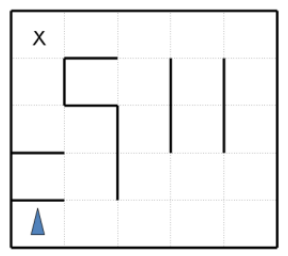
\includegraphics[width=0.3\linewidth]{figures/e1_maze.png}
\end{figure}

Consider a car agent which has to exit a maze. At all time-steps, the agent points at direction $d \in$ (N, S, E, W). With a single action, the agent can either move forward at an adjustable velocity $v \in [0, V]$ or turn. The turning actions are \texttt{left} and \texttt{right}, which change the agent's direction by 90 degrees. Turning is only permitted when the velocity is zero (and leaves it at zero). The moving actions are \texttt{faster} and \texttt{slower}. The action \texttt{faster} increments the velocity by 1 and \texttt{slower} decrements the velocity by 1; in both cases the agent then moves a number of squares equal to its \emph{new} velocity. Any action that would result in a collision with a wall is illegal. Any action that would reduce $v$ below 0 or above a maximum speed $V$ is also illegal. The agent's goal is to find a plan which parks it (stationary) on the exit square using as few actions (time steps) as possible.

As an example, in the hereabove maze, if the agent is initially stationary, it might first turn to the east using \texttt{right}, then move one square east using \texttt{faster}, then two more squares east using \texttt{faster} again. However, the agent will have to slow to take the turn.

\begin{enumerate}
    \item For a grid of size $M \times N$, what is the size of the state space? Assume that all configurations are reachable from the starting state.

    \begin{solution}
        $N \times M \times 4 \times (V + 1)$
    \end{solution}

    \item What is the maximum branching factor of this problem? Assume that illegal actions are simply not returned by the successor function.

    \begin{solution}
        The maximum branching factor is 3, and this happens when the agent is stationary. While stationary, it can take the following 3 actions: \texttt{faster}, \texttt{left}, \texttt{right}.
    \end{solution}

    \item Is the Manhattan distance from the agent's location to the exit's location admissible?

    \begin{solution}
        No because it does not take the velocity of the agent into account. For instance, in a long straight path, the number of steps could be smaller than the number of squares.
    \end{solution}

    \item If we used an inadmissible heuristic in \Astar{} tree search, could it change the completeness of the search? And the optimality ?

    \begin{solution}
        With an inadmissible heuristic, \Astar{} will still find a final state if there exists a reachable one (complete), but it could stop the search before finding the optimal one (non optimal).
    \end{solution}

    \item State and motivate a non-trivial admissible heuristic for this problem.

    \begin{solution}
        Some examples of admissible heuristics are:
        \begin{itemize}
            \item The Manhattan distance divided by the max speed $V$.
            \item We can improve the above heuristic by adding the current velocity $v$, as the agent has to slow down to 0 before reaching its goal. This heuristic \emph{dominates} the first one as it is always larger (or equal), but is still admissible as it never overestimates the true forward cost.
        \end{itemize}
    \end{solution}

    \item Give a general advantage that an inadmissible heuristic might have over an admissible one.

    \begin{solution}
        The time to solve an \Astar{} tree search problem is a function of two factors: the number of nodes expanded, and the time spent per node.
        \begin{itemize}
            \item An inadmissible heuristic may be faster to compute, leading to a solution that is obtained faster due to less time spent per node.
            \item Admissible heuristics are sometimes too conservative (well below $h^*$). An inadmissible heuristic could be a better estimate of the true forward cost $h^*$ (although it will overestimate at times), thus expanding less nodes.
        \end{itemize}
        We lose the guarantee of optimality by using an inadmissible heuristic. However, sometimes, we may be okay with finding a suboptimal solution faster.
    \end{solution}
\end{enumerate}

\newpage

\section{Heuristics (CS188, Spring 2019)}

Consider a graph search problem where all edges have a unit cost and the optimal solution has cost $C^*$. Let $h(n)$ be a heuristic which is $\max \cbk{h^*(n) - k, 0}$, where $h^*(n)$ is the true forward cost of $n$ and $k \leq C^*$ is a non-negative constant.

\begin{enumerate}
    \item Is $h$ admissible?

    \begin{solution}
        Yes. If $h^* \geq k$, $h^* - k \leq h^*$, otherwise $0 \leq h^*$.
    \end{solution}

    \item Which of the following is the most reasonable description of how much more work will be done, \ie{} how many more nodes will be expanded, with heuristic $h$ compared to $h^*$, as a function of $k$?

    \begin{enumerate}
        \item Constant in $k$
        \item Linear in $k$
        \item Exponential in $k$
        \item Unbounded
    \end{enumerate}

    \begin{solution}
        With this heuristic, all nodes $n$ such that $h^*(n) \leq k$, \ie{} within distance $k$ from the objective, will have have a null heuristic. Assuming a node can have up to $p$ parents, there is at most $p^k$ such node and the algorithm will expand all of them, in the worst case. Thus, the additional work is exponential in $k$.
    \end{solution}
\end{enumerate}

\newpage

\section{Search algorithms}

\begin{figure}[h]
    \centering
    \scalebox{0.75}{\begin{tikzpicture}[node distance = 4cm]
        \node[state] (S) {S(tart)};
        \node[state] (A) [above right of=S] {A};
        \node[state] (B) [right of=A] {B};
        \node[state] (C) [below of=B] {C};
        \node[state] (D) [below right of=B] {D};
        \node[state] (G) [below of=D] {G(oal)};

        \path[-] (S) edge node[fill=white] {1} (A);
        \path[-] (S) edge node[fill=white] {12} (G);
        \path[-] (A) edge node[fill=white] {3} (B);
        \path[-] (A) edge node[fill=white] {1} (C);
        \path[-] (B) edge node[fill=white] {3} (D);
        \path[-] (C) edge node[fill=white] {1} (D);
        \path[-] (C) edge node[fill=white] {2} (G);
        \path[-] (D) edge node[fill=white] {3} (G);
    \end{tikzpicture}}
\end{figure}

For each of the following search algorithms, give the order in which states are expanded as well as the final path returned by the algorithm. If two nodes are in competition to be expanded, the conflict is resolved by alphabetical order.

\begin{enumerate}
    \item Depth-First search (DFS)

    \begin{solution}
        Expansion: S, A, B, D, C, G. Path: S, A, B, D, C, G.
    \end{solution}

    \item Breadth-First Search (BFS)

    \begin{solution}
        Expansion: S, A, G. Path: S, G.
    \end{solution}

    \item Uniform-Cost search (UCS)

    \begin{solution}
        Expansion: S, A, C, D, B, G. Path: S, A, C, G.
    \end{solution}

    \item Consider the following heuristics:
    \begin{table}[h]
        \centering
        \begin{tabular}{c|cc}
            \toprule
            State & $h_1$ & $h_2$ \\
            \midrule
            S & 5 & 4\\
            A & 3 & 2\\
            B & 6 & 6\\
            C & 2 & 1\\
            D & 3 & 3\\
            G & 0 & 0\\
            \bottomrule
        \end{tabular}
    \end{table}
    which one is not admissible? Why?

    \begin{solution}
        The heuristic $h_1$ is not admissible because the real cost from S to G is 4 which is smaller than 5.
    \end{solution}

    \item \Astar{} (with the admissible heuristic)

    \begin{solution}
        Expansion: S, A, C, G. Path: S, A, C, G.
    \end{solution}
\end{enumerate}

\newpage

\section{The hive (CS188, Spring 2019)}

The hive of insects needs your help. You control an insect in a rectangular maze-like environment of size $M \times N$, as shown on the Figure below. At each time-step, the insect can move into a free adjacent cell or stay in its current location. All actions have a unit cost.

\begin{figure}[h]
    \centering
    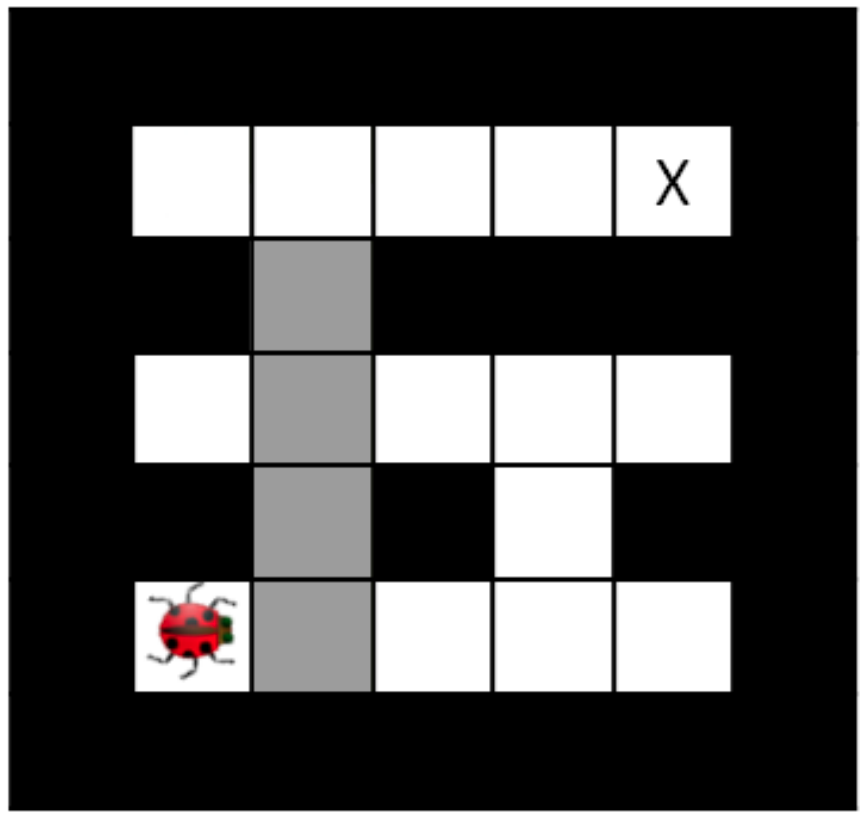
\includegraphics[width=0.3\linewidth]{figures/e1_hive.png}
\end{figure}

In this particular case, the insect must pass through a series of partially flooded tunnels, as illustrated by the gray cells on the map. The insect can hold its breath for $A$ time-steps in a row. Moving into a flooded cell requires your insect to consume 1 unit of air, while moving into a free cell refills its air supply.

\begin{itemize}
    \item Give a minimal state space for this problem (do not include extra information). You should answer for a general instance of the problem, not the specific map above.

    \begin{solution}
        The position of the insect  as well as the number of unit of air it has left. $s = (x, y, u_a) \in [1, M] \times [1, N] \times [1, A]$.
    \end{solution}

    \item Give the size of your state space.

    \begin{solution}
        $M\times N \times A$
    \end{solution}
\end{itemize}

\newpage

\section{Pacmen (INFO8006, January 2023)}

Pacman and his friends have decided to combine forces and go on the offensive, and are now chasing ghosts! In a grid of size $M \times N$, Pacman and $P - 1$ of his friends are moving around to collectively eliminate all of the ghosts in the grid by stepping on the same square as each of them. Moving into the same square as a ghost will eliminate it from the grid. At every turn, Pacman and his friends may choose one of the four (\texttt{north}, \texttt{south}, \texttt{east}, \texttt{west}) actions but may not collide with each other. In other words, any action that would result in two or more Pacmen occupying the same square will result in no movement for either of the Pacmen. Additionally, Pacman and his friends are \emph{indistinguishable} from each other. There are a total of $G$ ghosts, which are also indistinguishable from each other and cannot move.

Treating this as a search problem, we consider each configuration of the grid to be a state, and the goal state to be the configuration where all ghosts have been eliminated from the board. The cost of each turn (all Pacmen move once) is $1$. Below is an example starting state, as well as an example of goal state.

\begin{figure}[h]
    \centering
    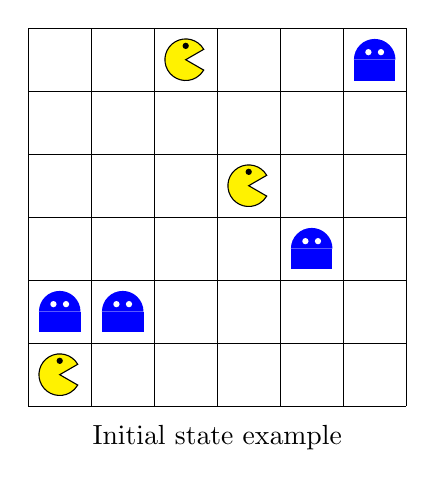
\begin{tikzpicture}[x=0.8cm, y=0.8cm]
        \draw (3, -0.5) node {Initial state example};
        \draw[step=1, black, thin] (0,0) grid (6,6);

        \draw[black, thin, fill=yellow] (0.5, 0.5) -- ++(30:0.33) arc (30:330:0.33) -- cycle;
        \fill[black] (0.5, 0.72) circle (0.05);

        \draw[black, thin, fill=yellow] (3.5, 3.5) -- ++(30:0.33) arc (30:330:0.33) -- cycle;
        \fill[black] (3.5, 3.72) circle (0.05);

        \draw[black, thin, fill=yellow] (2.5, 5.5) -- ++(30:0.33) arc (30:330:0.33) -- cycle;
        \fill[black] (2.5, 5.72) circle (0.05);

        \path[fill=blue] (1.5, 1.5) -- ++(0:0.33) arc (0:180:0.33) --
        cycle;
        \path[fill=blue] (1.5-0.33,1.5) rectangle ++(2*0.33,-0.33);
        \fill[white] (1.6, 1.62) circle (0.05);
        \fill[white] (1.4, 1.62) circle (0.05);

        \path[fill=blue] (0.5, 1.5) -- ++(0:0.33) arc (0:180:0.33) --
        cycle;
        \path[fill=blue] (0.5-0.33,1.5) rectangle ++(2*0.33,-0.33);
        \fill[white] (0.6, 1.62) circle (0.05);
        \fill[white] (0.4, 1.62) circle (0.05);

        \path[fill=blue] (4.5, 2.5) -- ++(0:0.33) arc (0:180:0.33) --
        cycle;
        \path[fill=blue] (4.5-0.33,2.5) rectangle ++(2*0.33,-0.33);
        \fill[white] (4.6, 2.62) circle (0.05);
        \fill[white] (4.4, 2.62) circle (0.05);

        \path[fill=blue] (5.5, 5.5) -- ++(0:0.33) arc (0:180:0.33) --
        cycle;
        \path[fill=blue] (5.5-0.33,5.5) rectangle ++(2*0.33,-0.33);
        \fill[white] (5.6, 5.62) circle (0.05);
        \fill[white] (5.4, 5.62) circle (0.05);
    \end{tikzpicture}
    \hspace{1cm}
    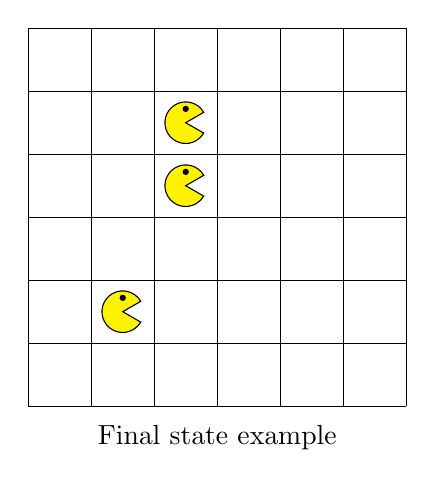
\begin{tikzpicture}[x=0.8cm, y=0.8cm]
        \draw (3, -0.5) node {Final state example};
        \draw[step=1, black, thin] (0,0) grid (6,6);

        \draw[black, thin, fill=yellow] (1.5, 1.5) -- ++(30:0.33) arc (30:330:0.33) -- cycle;
        \fill[black] (1.5, 1.72) circle (0.05);

        \draw[black, thin, fill=yellow] (2.5, 3.5) -- ++(30:0.33) arc (30:330:0.33) -- cycle;
        \fill[black] (2.5, 3.72) circle (0.05);

        \draw[black, thin, fill=yellow] (2.5, 4.5) -- ++(30:0.33) arc (30:330:0.33) -- cycle;
        \fill[black] (2.5, 4.72) circle (0.05);
    \end{tikzpicture}
\end{figure}

Suppose that Pacman has no friends ($P=1$).

\begin{enumerate}
    \item What is the size of the minimal state space representation? Explain your answer.

    \begin{solution}
        The state $s$ is fully described with the position of Pacman and a boolean for each ghost (eaten or not). The size of the state space is therefore $M \times N \times 2^G$. We don't need to save the position of the ghosts within the state because they never change.
    \end{solution}

    \item Explain whether each of the following heuristics is admissible, consistent, neither, or both.
    \begin{itemize}[leftmargin=*]
        \item $h_1(s) =$ the sum of the Manhattan distances from Pacman to every ghost.
        \item $h_2(s) =$ the number of ghosts times the maximum Manhattan distance between Pacman and any of the ghosts.
        \item $h_3(s) =$ the number of remaining ghosts.
    \end{itemize}

    \begin{solution}
        A heuristic $h(s)$ is admissible if $0 \leq h(s) \leq h^*(s)$ where $h^*(s)$ is the true forward cost. A heuristic is consistent if $h(s) - h(s') \leq c(s, s')$, where $c(s, s')$ is the cost from $s$ to $s'$. Note that a non-admissible heuristic cannot be consistent.

        In the following state $s$, $h_1(s) = 2 + 3 + 4$ and $h_2(s) = 3 \times 4$ are larger than $h^*(s) = 4$ (not admissible) and $h_1(s) - h_1(s') = 3$ and $h_2(s) - h_2(s') = 3$ are larger than $c(s, s') = 1$ (not consistent).

        \begin{center}
        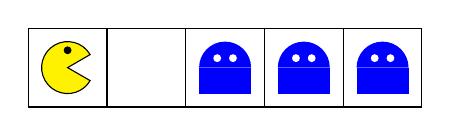
\begin{tikzpicture}
            \draw[step=1, black, thin] (0,0) grid (5,1);

            \draw[black, thin, fill=yellow] (0.5, 0.5) -- ++(30:0.33) arc (30:330:0.33) -- cycle;
            \fill[black] (0.5, 0.72) circle (0.05);

            \path[fill=blue] (2.5, 0.5) -- ++(0:0.33) arc (0:180:0.33) --
            cycle;
            \path[fill=blue] (2.5-0.33,0.5) rectangle ++(2*0.33,-0.33);
            \fill[white] (2.6, 0.62) circle (0.05);
            \fill[white] (2.4, 0.62) circle (0.05);

            \path[fill=blue] (3.5, 0.5) -- ++(0:0.33) arc (0:180:0.33) --
            cycle;
            \path[fill=blue] (3.5-0.33,0.5) rectangle ++(2*0.33,-0.33);
            \fill[white] (3.6, 0.62) circle (0.05);
            \fill[white] (3.4, 0.62) circle (0.05);

            \path[fill=blue] (4.5, 0.5) -- ++(0:0.33) arc (0:180:0.33) --
            cycle;
            \path[fill=blue] (4.5-0.33,0.5) rectangle ++(2*0.33,-0.33);
            \fill[white] (4.6, 0.62) circle (0.05);
            \fill[white] (4.4, 0.62) circle (0.05);
        \end{tikzpicture}
        \end{center}

        Conversely, for any state $s$, $h_3(s)$ is a lower bound for the number of remaining turns (admissible) and $h_3(s) - h_3(s')$ is either $0$ or $1$, which is lower than $c(s, s') = 1$ (consistent).
    \end{solution}
\end{enumerate}

Suppose that Pacman has exactly one less friend than the number of ghosts ($P=G$).

\begin{enumerate}[resume]
    \item What is the size of the minimal state space representation? Explain your answer.

    \begin{solution}
        The state $s$ is fully described with the position of each Pacman and a boolean for each ghost (eaten or not). The size of the state space is therefore (at most) $(M \times N)^P \times 2^G$. Alternatively, the position of the Pacmen can also be represented by $M \times N$ booleans, which would result in $2^{M \times N} \times 2^G$ states. Depending on $P$, the latter representation could be smaller or larger.
    \end{solution}

    \item Explain whether each of the following heuristics is admissible, consistent, neither, or both.
    \begin{itemize}[leftmargin=*]
        \item $h_4(s) =$ the largest of the Manhattan distances between each Pacman and its closest ghost.
        \item $h_5(s) =$ the smallest of the Manhattan distances between each Pacman and its closest ghost.
        \item $h_6(s) =$ the number of remaining ghosts.
        \item $h_7(s) =$ the number of remaining ghosts divided by $P$.
     \end{itemize}

     \begin{solution}
        $h_4$ and $h_6$ could be larger than the number of remaining turns (not admissible, not consistent). $h_5$ and $h_7$ are admissible and consistent.
    \end{solution}
\end{enumerate}

\newpage

\startquiz

The \Astar algorithm, in its graph version is ...
\begin{itemize}
    \item always optimal.
    \item always optimal if the heuristic is admissible.
    \solitem always optimal if the heuristic is consistent.
    \item never optimal when there are cycles.
\end{itemize}

In a fully observable but stochastic game, if a simple reflex agent is presented the same state several times, it will ...
\begin{itemize}
    \solitem take the same action every time.
    \item take a different action every time.
    \item take a different action most of the time.
    \item take the same action most of the time.
\end{itemize}

Which of the following statements about heuristics are true ?
\begin{itemize}
    \item $h(n) = 0 \ \forall n$ can speed up \Astar compared to UCS.
    \item If a heuristic is admissible, it is guaranteed to be consistent.
    \item The average step cost $h(n) = \frac{1}{\#a}\sum_a c(n,a,n')$ is admissible.
    \solitem The true remaining cost dominates all admissible heuristics.
\end{itemize}

The black-jack game is ...
\begin{itemize}
    \item discrete, multi-agent and deterministic.
    \solitem partially-observable, stochastic and multi-agent.
    \item partially-observable, episodic and single-agent.
    \item None of the above.
\end{itemize}

A goal-based planning agent ...
\begin{itemize}
    \item cannot decide which action to take next if the transition model is wrong.
    \item ignores the consequences of its actions to take decisions.
    \solitem can be implemented using the greedy search algorithm.
    \item need a Markovian system to be optimal.
\end{itemize}
\end{document}
